\section{ Einleitung }

% \begin{frame}
% 	\frametitle{ Womit beschäftige ich mich? }
%     \begin{itemize}
%         \item Supraleitung beschrieben über BCS-Theorie 
%         \item Wende auf Bienenwabengitter, Gitterstrukur z.B. von Graphen an
%         \item Ziel: Das Auftreten von Supraleitung und dessen Begrenzungen in dem Bienenwabengitter zu untersuchen
%     \end{itemize}
% \end{frame}
\begin{frame}
    \frametitle{Übersicht}
    \begin{itemize}
        \item Einleitung
        \item Modell
        \item Ergebnisse
        \item Zusammenfassung und Ausblick
    \end{itemize}
\end{frame}

\begin{frame}
    \frametitle{Supraleitung}
    \begin{itemize}
        % \item Supraleitung mega cool
        % \item kann das:
        % \item kann aber auch das:
        % \item wow!
        \item 
    \end{itemize}
\end{frame}

% \begin{frame}
%     \frametitle{BCS-Theorie -- Ein Überblick (1)}
%     \begin{minipage}[c]{0.7\textwidth}
%         \begin{itemize}
%             \item Beschreibung konventioneller Supraleitung 
%             \item Grundlegender Mechanismus: Elektron-Phonon-Wechselwirkung 
%             \begin{itemize}
%                 \item[$\rightarrow$] effektive, phononenvermitelte Elektron-Elektron-Anziehung 
%             \end{itemize}
%             \item Bildung von Cooper-Paaren 
%             \begin{itemize}
%                 \item[$\rightarrow$] Kopplung von Zuständen $(\vk, \up)$ und $(-\vk, \down)$ 
%                 \item[$\rightarrow$] gebundene ``bosonische'' Quasiteilchen mit Impuls $0$ und Spin $0$
%             \end{itemize}
%             \item attraktive Wechselwirkung führt zu ``Cooper-Instabilität''
%             \begin{itemize}
%                 \item[$\rightarrow$] Bildung von Cooper-Paaren energetisch begünstigt
%                 \item[$\rightarrow$] für $T<T_C$ makroskopischer Quantenzustand (Supraleitung)
%             \end{itemize}
%         \end{itemize}
%     \end{minipage}
%     \begin{minipage}[c]{0.29\textwidth}
%         \begin{figure}
%             \centering
%             
\includegraphics[width=0.8\textwidth]{images/cooperall.png}
%             \caption{Anregung einer Gitterpolarisation durch ein Elektron~\cite{czycholl_theoretische_2017}.}
%             % \label{<label>}
%         \end{figure}
%     \end{minipage}
% \end{frame}

\begin{frame}
    \frametitle{BCS-Theorie  -- Ein Überblick (1)}
    \begin{itemize}
        \item Elektron-Phonon-Wechselwirkung 
            \begin{itemize}
                \item[$\rightarrow$] effektive, phononenvermitelte Elektron-Elektron-Anziehung 
            \end{itemize}
        \item Bildung von Cooper-Paaren 
        \begin{itemize}
            \item[$\rightarrow$] Kopplung von Zuständen $(\vk, \up)$ und $(-\vk, \down)$ 
            \item[$\rightarrow$] gebundene ``bosonische'' Quasiteilchen mit Impuls $0$ und Spin $0$
        \end{itemize}
    \end{itemize}
    \begin{figure}[htbp]
        \centering
        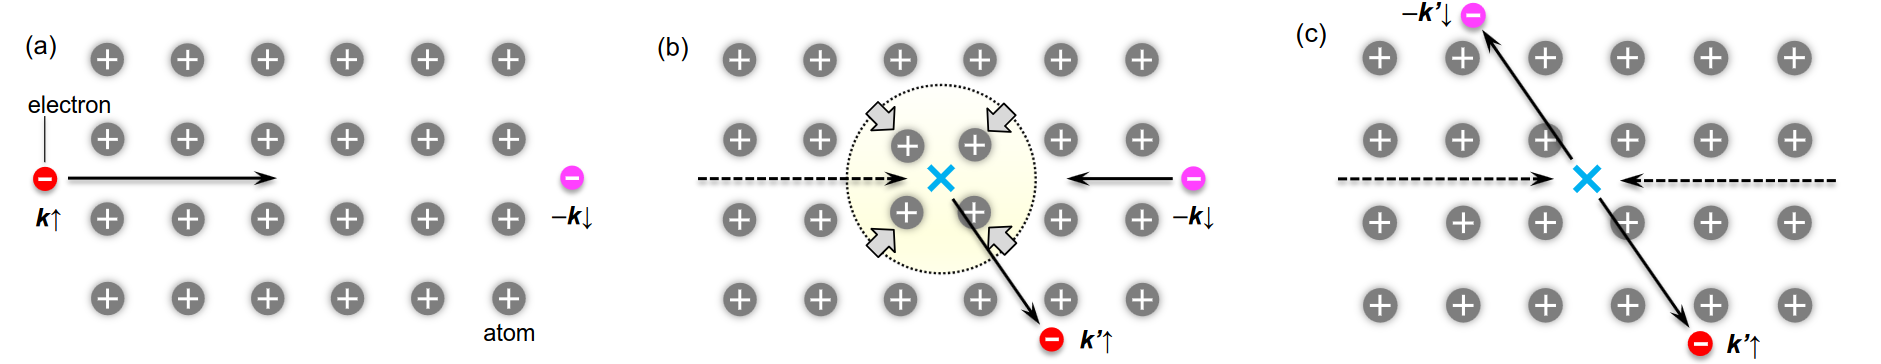
\includegraphics[width=\textwidth]{images/cooperall2.png}
        \caption{Bildung von Cooper-Paaren~\cite{hiroi_introduction_2026}.}
        % \label{<label>}
    \end{figure}
\end{frame}

\begin{frame}
    \frametitle{BCS-Theorie -- Ein Überblick (2)}
    \begin{itemize}
        \item attraktive Wechselwirkung führt zu ``Cooper-Instabilität''
            \begin{itemize}
                \item[$\rightarrow$] Bildung von Cooper-Paaren energetisch begünstigt
                \item[$\rightarrow$] für $T<T_C$ makroskopischer Quantenzustand (Supraleitung)
            \end{itemize}
        \item Beschreibung durch BCS-Hamiltonian 
        \begin{align*}
            \oH_\text{BCS} = -\frac{U}{N} \sum_{\vk, \vk'} \ofed{\vk', \up} \ofed{-\vk', \down} \ofe{-\vk, \down} \ofe{\vk, \up} \Theta(\hbar \omega_D - \abs{\epsilon_\vk - E_F}) \Theta(\hbar \omega_D - \abs{\epsilon_{\vk'} - E_F})
        \end{align*}
        \begin{itemize}
            \item[$\rightarrow$] nur Elektronen mit $\epsilon_\vk \in [E_F - \hbar \omega_D, E_F + \hbar \omega_D]$ tragen bei 
            \item[$\rightarrow$] Wechselwirkungsstärke ist konstant (unabhängig von $\vk$)
        \end{itemize}
    \end{itemize}
\end{frame}

% \begin{frame}
%     \frametitle{Bienenwabengitter}
%     \begin{figure}
%         \centering
%         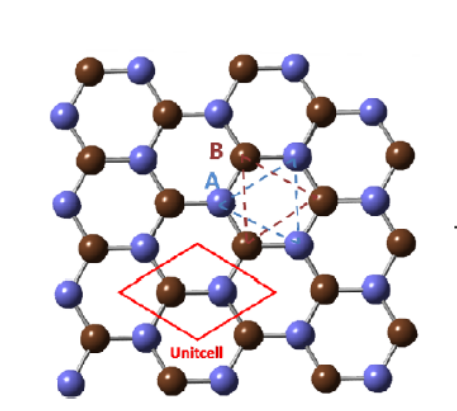
\includegraphics[width=0.5\textwidth]{images/gitter.png}
%         \caption{Quelle aus dem Skript von Uhrig (Bitte original)}
%         % \label{<label>}
%     \end{figure}
% \end{frame}

\begin{frame}
    \frametitle{Bienenwabengitter -- Überblick}
    \begin{minipage}[t]{0.6\textwidth}
        \begin{itemize}
            \item hexagonales 2D-Gitter $=$ 2 trigonale Untergitter A und B
            \begin{itemize}
                \item[$\rightarrow$] zweiatomige Basis
            \end{itemize}
            \item Nächste-Nachbar-Vektoren 
            \begin{align*}
                \vd{1} &= \frac{a}{2} \begin{pmatrix}1 \\ \sqrt{3}\end{pmatrix} & \vd{2} &= \frac{a}{2} \begin{pmatrix}1 \\ -\sqrt{3}\end{pmatrix}, & \vd{3} &= a \begin{pmatrix}-1 \\ 0\end{pmatrix}
            \end{align*}
            \item Gitterstruktur von bspw. Graphen, Bornitrid (h-BN), $\mathrm{MoS_2}$, etc.
        \end{itemize}
    \end{minipage}
    \begin{minipage}[t]{0.39\textwidth}
        \begin{figure}
            \centering
            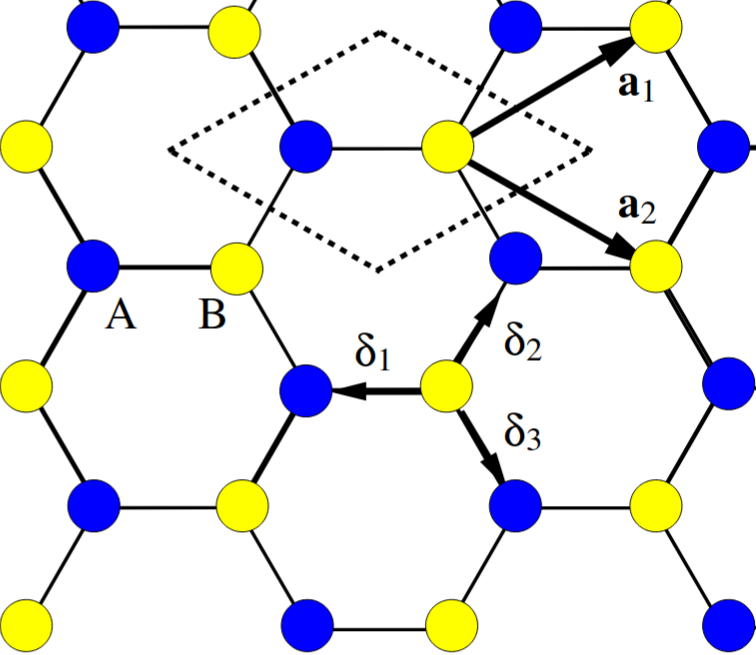
\includegraphics[width=\textwidth]{images/gitter3.png}
            \caption{Bienenwabengitter~\cite{maksymiuk_tunable_2025}.}
            % \label{<label>}
        \end{figure}
    \end{minipage}
\end{frame}

\begin{frame}
    \frametitle{Bienenwabengitter -- Tight-Binding-Modell}
    \begin{itemize}
        \item Beschreibung über Nächste-Nachbar Tight-Binding-Modell
        \begin{align*}
            \oH_{\text{TB}} &= -t \sum_{\expval{\vec{R}, \vec{R}'}} \oad{\vec{R}} \ob{\vec{R}'} + \hc
        \end{align*}
        \item $\oA_{\alpha}$ und $\oB_{\beta}$ erfüllen die Antikommutatorrelationen
        \begin{align*}
            \anticommute{\oad{\alpha}, \oa{\beta}} &= \anticommute{\obd{\alpha}, \ob{\beta}} = \delta_{\alpha \beta} 
        \end{align*}
    \end{itemize}
\end{frame}